% arara: xelatex: { shell : yes }
% arara: biber
% arara: xelatex: { shell : yes }
% arara: xelatex: { shell : yes }

% options:
% thesis=B bachelor's thesis
% thesis=M master's thesis
% Czech thesis in Czech language
% Slovak thesis in Slovak language
% English thesis in English language
% hide links remove color boxes around hyperlinks

\documentclass[thesis=B,czech]{template/FITthesis}[2019/12/23]

\usepackage[utf8]{inputenc} % LaTeX source encoded as UTF-8
\usepackage{dirtree} %directory tree visualization

\usepackage{lipsum}
\usepackage{xevlna}
\usepackage{pdfpages}
\usepackage{minted}
\usemintedstyle{friendly}


\usepackage{chngcntr}
\counterwithin{listing}{chapter}

\usepackage[htt]{hyphenat}
\usepackage{caption}

\usepackage[style=iso-numeric]{biblatex}
\addbibresource{ref.bib}

\usepackage{float}

\def\UrlBreaks{\do\/\do\-\do\_}


\RequirePackage{xcolor} 
\newcommand{\todo}[1]{\textcolor{red}{\textbf{[[#1]]}}}

% % % % % % % % % % % % % % % % % % % % % % % % % % % % % % 
% ODTUD DAL VSE ZMENTE
% % % % % % % % % % % % % % % % % % % % % % % % % % % % % % 

\department{Katedra softwarového inženýrství}
\title{Návrh a implementace knihovny pro automatizaci testů verifikace průmyslové komunikace}
\authorGN{Martin} %(křestní) jméno (jména) autora
\authorFN{Štěpánek} %příjmení autora
\authorWithDegrees{Martin Štěpánek} %jméno autora včetně současných akademických titulů
\author{Martin Štěpánek} %jméno autora bez akademických titulů
\supervisor{Ing.\,{}Miroslav Dušek}
\acknowledgements{Doplňte, máte-li komu a za co děkovat. V~opačném případě úplně odstraňte tento příkaz.}

\abstractCS{Tato bakalářská práce se zabývá návrhem a implementací knihovny pro automatizaci testů verifikace průmyslové komunikace. Vytvořená knihovna funguje jako doplněk do testovacího frameworku MSTest, za pomocí nehož je knihovna následně propojena se serverem Azure DevOps. Ten následně může jednotlivé testy registrovat a automaticky spouštět. Práce také ukazuje open-source knihovny pro průmyslové protokoly ModbusTCP a EtherNet/IP, které jsou vhodné k využití současně s testovací knihovnou, a za pomocí jedné z těchto knihoven následně demonstruje funčknost vytvořeného řešení. Na závěr práce zhodnocuje ekonomický přínos vytvořeného řešení.}

\abstractEN{This bachelor's thesis is focused on design and implementation of test automation library for verification of industry fieldbus communication. This library works as add-in to testing framework MSTest, which enables connection with Azure DevOps. Azure DevOps then can register each of the tests and automatically execute them. This thesis also shows open-source libraries for fieldbuses ModbusTCP and EtherNet/IP, which are suitable for use together with the created test library. Thesis also demonstrates the funcionality of the created test library, with the help of one of the open-source library for fieldbus. Lastly the thesis evalutes the created solution from the economic point of view.} 

\placeForDeclarationOfAuthenticity{V~Praze}
\declarationOfAuthenticityOption{4} %volba Prohlášení (číslo 1-6)
\keywordsCS{softwarové testování, automatizace testů, verifikace průmyslová komunikace, MSTest, ModbusTCP, EtherNet/IP}
\keywordsEN{software testing, test automation, verification of fieldbus communication, MSTest, ModbusTCP, EtherNet/IP}
% \website{http://site.example/thesis} %volitelná URL práce, objeví se v tiráži - úplně odstraňte, nemáte-li URL práce

\begin{document}

\begin{introduction}
\lipsum[1-5]
\end{introduction}


\chapter{Cíl práce}\label{chap:cil}
Cílem této práce je navrhnout a implementovat knihovnu, která umožní automatizovat testy verifikace průmyslové komunikace. 
Součástí této knihovny má být:
\begin{itemize}
    \item služba, která bude řídit testovací běh,
    \item rozhraní, které umožní implementaci knihovny na testovaném zařízení,
    \item protokol, který bude definovat komunikaci mezi službou a testovanými zařízeními.
\end{itemize}
Vytvořená knihovna poté má být propojena s Azure DevOps serverem tak, aby Azure DevOps server mohl následně automaticky spouštět testy. Azure DevOps server následně má být schopen spuštěné testy vyhodnotit a poskytnout uživateli informaci o průběhu jednotlivých testů. 
Dalším cílem je provést výzkum dostupných open-source knihoven pro průmyslové protokoly ModbusTCP a EtherNet/IP a vybrat vhodné kandidáty na implementaci do této knihovny. 
Součástí této práce má též být demonstrace použití vytvořené testovací knihovny, kde bude využit jeden z průmyslových protokolů. V neposlední řadě je cílem zhodnotit vytvořené řešení a jeho přínosy z pohledu projektového řízení.

\chapter{Teoretická část}\label{chap:teorie}

\section{Testování}

Testování je podstatnou součástí vývoje produktu a jeho softwaru. Cílem testování není pouze odhalení chyb v softwaru, ale také verifikace a validace softwaru. Validací softwaru kontrolujeme, zda software odpovídá specifikacím a je tím, co zákazník chtěl. Verifikací kontrolujeme správnost softwaru, tedy kontrolujeme, že systém ve vytvořených situacích se chová dle očekávání a specifikace. \cite{singh2012software}

Testování softwaru je zároveň dovednost. Při testování musí tester vybrat z nekonečného množství možných testů nějaký konečný počet, který nejlépe reprezentuje danou problematiku a pokrývá co největší možnou množinu všech možných případů. Zároveň musí vzít v potaz náročnost na vytvoření testu a na rigidnost vytvořeného testu proti změnám v softwaru. Tyto faktory poté ovlivňují i náklady na testování. \cite{fewster1999software}

Od testování softwaru lze také odvodit kvalitu softwaru. Kvalita softwaru se dá určit tím, jak moc vytvořený software odpovídá zadaným specifikacím~\cite{software_quality}. Tyto informace jsou poté velmi důležité pro managment. Díky nim může vyhodnocovat současný stav vývoje a upravovat plán na vývoj. 

Testování zároveň zvyšuje důvěru ve vyvíjený softwaru. Každý dobře navržený test snižuje šanci, že v softwaru existuje nepodchycená chyba. S každým rozsáhlým testováním se tato důvěra zvyšuje. \cite{fewster1999software}

\subsection{Rozdělení testů}

I když primární cíl testování je jednotný, přístupů k testování je několik. Vhodnost jednotlivých přístupů se mění na základě testované komponenty. Tyto přístupy se dají podle \cite{luo2001software} rozdělit do několika kategorií.

\subsubsection{Podle znalosti komponenty}

Testování se dá rozdělit podle přístupu k informacím, které o komponentách softwaru/systému víme. Tyto typy jsou:

\begin{description}
    \item[Black box testování] Nazýváno taktéž funkční testování. Na software se pohlíží jako na tzv. černou skříňku. O komponentě nebo celku nic nevíme a testujeme na základě funkcionálních požadavků, návrhu, specifikací nebo uživatelské dokumentace. 
    \item[White box testování] Se znalostí implementace testované části se snažíme vytvořit takové testy, které způsobí spouštění určitých částí testované komponenty. Cílem je co největší pokrytí testování dané komponenty.
    \item[Grey box testování] Kombinace Black box a White box testování. Při testování máme nějakou znalost implementace komponenty, ale je nižší, než při White box testování. \cite{khan2010different}
\end{description}

\subsubsection{Podle částí vývoje}

Testování podle částí vývoje se přibližuje vývojovému cyklu. Tyto kategorie jsou:  

\begin{description}
    \item[Testování jednotlivých částí] Více známé pod anglickým pojmem \uv{Unit testing}. Je to nejnižší úroveň testování. Testuje jednotlivé komponenty systému samostatně.
    \item[Integrační testování] Testování dvou a více komponent, které spolu vytváří nějaký větší celek softwaru. Často také využíván při testování částí, které nelze samostatně testovat.
    \item[Systémové testování] Testování softwaru jako celku. Testování se směřuje na testování funkčních požadavků. Zároveň je možno vyhodnocovat další požadavky na systém, jako spolehlivost, bezpečnost, atd.
    \item[Akceptační testování] U toho testování se systém dostane do rukou zákazníkovi/uživatelům. Cílem je otestování produktu u uživatelů softwaru a získání jejich zpětné vazby. 
\end{description}

Propojení testů a vývojového cyklu je dobře znázorněno na tzv. V-modelu, který můžeme vidět na obrázku \ref{fig:vmodel}. Na tomto modelu, nazývaném podle svého tvaru, můžeme vidět jednotlivé typy stádia vývoje a jejich korespondující ověřování v závislosti na čase.

\begin{figure}[htbp]
    \centering 
    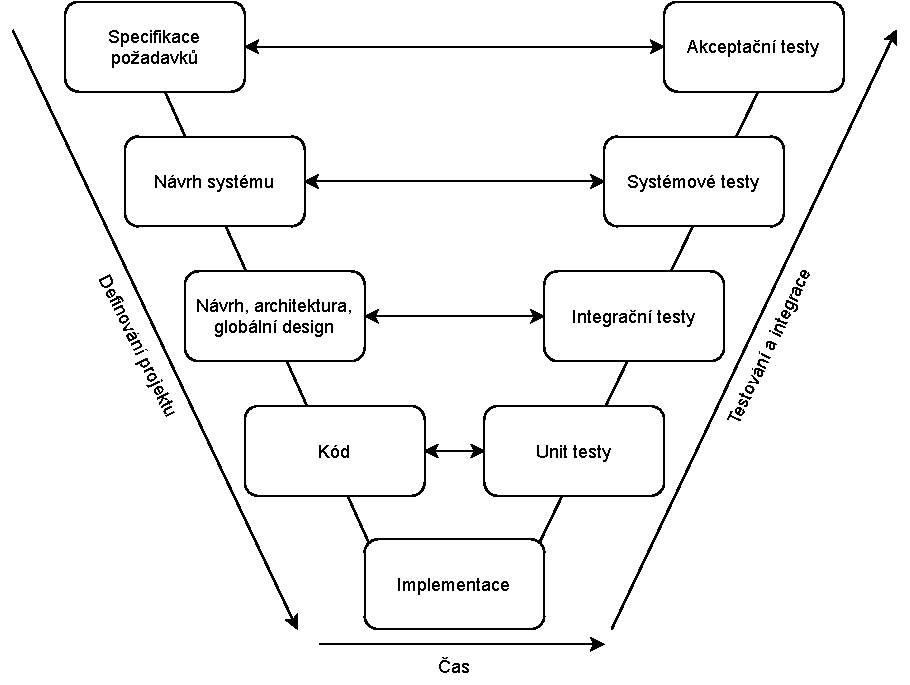
\includegraphics[width=0.9\textwidth]{assets/img/vmodel.pdf}
    \caption{V-model}
    \source{Vytvořeno dle předlohy z \cite{fewster1999software}}
    \label{fig:vmodel}
\end{figure}


\section{Automatizace testování}

Automatizace testování je odlišná od samotného testování. Automatizace testu neurčuje samotnou kvalitu testu. Pokud automatizujeme test, který nepřináší žádné nové benefity vývoji softwaru, tak poté dostaneme jeho výsledek pouze rychleji. \cite{fewster1999software} Proto tvorba testů je minimálně stejně důležitá, ne-li důležitější, jako samotná jejich automatizace. Automatizování je ale v mnoha ohledech v dnešní době standardem při testování, a to především díky jeho výhodám. Mezi tyto výhody podle \cite{fewster1999software} patří:

\begin{description}
    \item[Častější testování] S automatizací jsme schopni testovat software mnohem častěji, než při manuálním testování. Software může být testován například při každé jeho změně. Toto manuálně je velmi náročné, už jenom kvůli vysokému požadavku na lidské zdroje.  
    \item[Ulehčení testování] Test, který bude požadovat k jeho uskutečnění 200 uživatelů, není nemožný provést manuálně. S automatizací ale můžeme vstupy těchto uživatelů simulovat a tím celé testování zjednodušit.  
    \item[Lepší využití zdrojů] Tester je kvalifikovaný člověk a jeho využití na opakované vkládání vstupů a ověřování výstupů může být v některých případech plýtváním jeho časem.
    Taktéž při manuálním testování můžeme vyžadovat více účastníků testování, kteří všichni si musí vyhradit čas na testování. Díky automatizaci můžeme tyto zdroje využít víc efektivněji. Tester se například díky automatizaci může více soustředit na vytváření nových testů.
    \item[Konzistence] Při automatizaci testování každý běh testu proběhne naprosto identicky. Stejně jako ve vývoji, i v testování může dojít k lidské chybě. Díky automatizaci se šance lidské chyby snižuje. Toto zvyšuje konzistenci testování, než když se testy provádějí manuálně.
    \item[Snížení doby testování] Jednou automatizované testy mohou být provedeny mnohem rychleji a efektivněji, než při jejich manuálním spuštění. Toto způsobuje snížení potřebné doby na testování.
\end{description}

Automatizované testování následně může podporovat další procesy během vývoje. Mezi tyto procesy patří například proces kontinuální integrace nebo proces kontinuálního doručení softwaru. Proces kontinuální integrace se zaměřuje na integrování jednotlivých upravovaných částí do celkového softwaru. Oproti tomu proces kontinuálního doručení softwaru se zaměřuje na to, aby software vždy byl v takovém stavu, aby mohl být doručen zákazníkovi, nebo nasazen. \cite{ci_cd}

\section{Azure DevOps}

Azure DevOps server poskytuje vývojářům služby, které pomáhají při vývoji softwaru. Jeho cílem je podporovat jednotlivé procesy vývoje, což poté zrychluje vývoj softwaru. \cite{azure_devops} V této práci budu využívat několik služeb, které Azure DevOps server nabízí. Tyto služby budou:

\begin{description}
    \item[Azure Repos] Azure Repos je sada nástrojů, která umožňuje správu jednotlivých verzí softwaru. V této práci budeme používat systém správy verzí Git, který je Azure Repos podporovaný. \cite{azure_repos}
    \item[Azure Pipelines] Azure Pipelines umožňuje automaticky kompilovat a testovat vyvíjený software. Tím také podporuje procesy kontinuální integrace, kontinuálního nasazení softwaru nebo kontinuálního testování. \cite{azure_pipelines}
    \item[Azure Test Plans] Azure Test Plans přináší sadu nástrojů, které umožnují spravovat testování softwaru. Tyto nástroje umožňují správu testovacích sad a jednotlivých testů, ať už manuálních nebo automatizovaných. \cite{azure_test_plans}
    \item[Azure Artifacts] Azure Artifacts umožňuje publikování a verzování různých typů balíčků. Následně tato správa těchto balíčků může být využita při vydání těchto balíčků. Mezi podporované balíčky patří například NuGet, Maven nebo npm. Zároveň skrz Azure Artifact můžeme publikovat data z Azure Pipelines. \cite{azure_artifacts}
\end{description}

Azure DevOps server využívá při delegování úkolů tzv. agenty. Agent je výpočetní infrastruktura s nainstalovaným softwarem agenta, který pracuje na jedné určité úloze \cite{agent_docs}. Agent následně provádí například jednotlivé úkony definované v Azure Pipelines, jako kompilace, testování atd.

\section{Framework MSTest}

Framework MSTest je výchozí testovací framework, který je integrován do IDE Visual Studio. Díky tomu je také často nazýván jako \uv{Visual Studio Unit Testing Framework}. Framework započal jako nástroj spouštěný z příkazové řádky, který následně prováděl testování. Díky implementaci do Visual Studia je tento framework často preferován vývojáři, kteří používají Visual Studio pro vývoj. 

MSTest framework přináší nástroje, které jsou potřeba k verifikaci a validaci softwaru. V dnešní době framework MSTest V2 je open-source projekt, který je stále rozvíjen. Mezi jeho výhody patří podpora napříč platformami a rozšiřitelnost. \cite{mstest_descr}


\section{Průmyslová komunikace}\label{sec:fieldbus}

Při řešení průmyslové komunikace se často objevuje slovo \textit{fieldbus}. Běžný význam tohoto slova je \uv{Síť, která propojuje průmyslová zařízení jako kontrolery, PLC, regulátory atd.} \cite{fieldbus_thomesse}. Vznik těchto sítí je úzce spojený s historií vývoje informačních technologií. V době, kdy začali tyto sítě vznikat, nebyli dostupné komunikační technologie, jako dnes. Dostupné informační a telekomunikační sítě té doby nemohli uspokojit potřeby průmyslových sítí na deterministickou, spolehlivou a efektivní komunikaci \cite{future_of_ind_com}. 

V dobách vzniku těchto komunikačních protokolů bylo pro fyzické připojení využíváno různých protokolů -- například RS-485. Nedostatkem těchto protokolů avšak byli vysoké implementační náklady. S růstem popularity standardu IEEE 802.3 -- dnes často nazýván Ethernet -- se začalo zkoumat možné použití tohoto standardu při průmyslové komunikaci. Odborníci došli k závěru, že je možné při průmyslové komunikaci v reálném čase využít tento standard \cite{lee_ethernet_fieldbus}. V dnešní době je Ethernetový standard hojně využíván při přenosu průmyslové komunikace.


\subsection{Protokol Modbus}
Modbus je průmyslový komunikační protokol, který je umístěn na aplikační vrstvě ISO/OSI modelu. Tento protokol, vytvořený v roce 1979, umožňuje komunikaci typu klient-server mezi zařízeními na různých typech sítí a sběrnic. 

Protokol definuje strukturu zprávy (tzv. PDU -- Protocol Data Unit) nezávisle od komunikační vrstvy. Tato zpráva se avšak může rozšířit, v závislosti na způsobu přenosu této zprávy. V závislosti na typu sítě je poté tato zpráva rozšířena o další údaje. Tento celek se poté označuje jako ADU -- Application Data Unit. Tuto celou strukturu můžeme vidět znázorněnou na obrázku \ref{fig:modbus_frame}.~\cite{modbus}

\begin{figure}[htbp]
    \centering 
    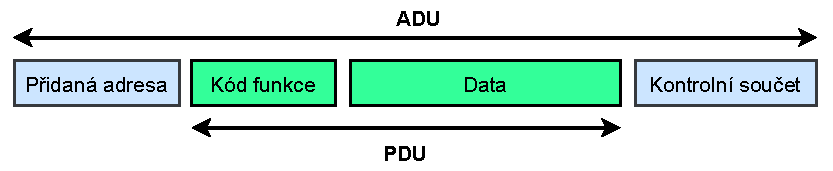
\includegraphics[width=\textwidth]{assets/img/modbusframe.pdf}
    \caption{Obecné znázornění jednoho rámce protokolu Modbus}
    \source{Vytvořeno dle předlohy z \cite{modbus}}
    \label{fig:modbus_frame}
\end{figure}

Podporované služby jsou definováno funkčními kódy, které jsou součástí požadavku. Kód funkce je uložen v jednom bajtu a tedy rozsah možných kódu je 1-255 (0 je nevalidní), kde rozsah 128-255 je rezervován pro chybové zprávy. Data zprávy poté slouží k upřesnění operace definované funkčním kódem. V určitých situacích muže postačovat v provedení operace funkční kód, data zprávy poté mají nulovou délku.

Modbus používá komunikaci požadavek-odpověď. Na požadavek klienta server odpovídá zprávou, kterou značí úspěch či neúspěch operace. V případě úspěchu server odesílá zpět zprávu se stejným funkčním kódem jako byl požadavek. V opačném případě odesílá zpět zprávu, která obsahuje stejný kód funkce jako byl kód funkce požadavku, ale tento kód má zároveň nastavený nejvýznamnější bit na 1. Zpráva v obou případech může poté obsahovat data, v závislosti na operacích. \cite{modbus}

V této práci se budu zaměřovat na použití protokolu ModbusTCP. Jak již z názvu vyplívá, ModbusTCP používá k přenosu zpráv protokol TCP/IP a Ethernet připojení. Zároveň používá stejnou komunikaci definovanou protokolem Modbus.

\subsection{Protokol EtherNet/IP}
Protokol EtherNet/IP (EtherNet/Industrial Protocol) je dalším dnes již široce používaným průmyslovým protokolem. Jak již z názvu vyplívá, protokol používá Ethernetový standard k propojení průmyslových zařízení. Ke komunikaci následně používá standardně používané protokoly TCP a UDP. Tento protokol byl poprvé představen v roce 2001 a od roku 2005 je standardizován. 

Protokol je umístěn na 5--7 vrstvě ISO/OSI modelu. V rámci sítě jsou jednotlivým uzlům přiřazeny předem definované profily. Profil reprezentuje typ zařízení se specifickými vlastnostmi. Profil zařízení a aplikační vrstva protokolu EtherNet/IP jsou vytvářeny protokolem CIP (Common Industrial Protocol). Tento protokol používá komunikaci na principu producent-konzument. Použitím společného protokolu CIP se následně dosahuje interoperability mezi všemi sítěmi, které ho podporují. 

Protokol CIP je objektově orientovaný. Každé zařízení je reprezentováno skupinou objektů. Každý z objektů obsahuje data, služby resp. příkazy a specifikaci funkcí. V rámci protokolu je poté definováno, jaké atributy musí každý objekt obsahovat.

Aplikační objekty obsahují data, které jsou specifická pro komunikující zařízeni. Výrobci mohou specifikovat i svoje vlastní objekty. Pro identifikaci dostupných objektů jsou sestaveny elektronické popisy zařízení, které obsahují potřebné informace ke konfiguraci zařízení v síti EtherNet/IP. 

Přenos v síti EtherNet/IP se odvíjí dle využitého protokolu pro přenos. Při použití protokolu TCP je přenos explicitní a je určen k přenosu typu žádost-odpověď mezi dvěma zařízeními. Naopak při použití protokolu UDP je přenos implicitní, který je pak určený pro cyklický přenos uživatelských a I/O dat. Komunikační model objektů CIP umožňuje lépe využít možnosti komunikačního kanálu. Přenos zprávy následně probíhá dle protokolu. Žadatel zahajuje komunikaci s cílovým zařízením odesláním žádosti k vytvoření komunikace, která obsahuje navrhované parametry spojení. Cílové zařízení následně odesílá potvrzení s přesnými parametry a navazuje spojení. Každé spojení je poté určeno identifikátorem. \cite{ethernet_ip}

\section{Testovaný produkt}

Hlavním cílem této práce je vytvoření testovací knihovny pro řadu zařízení SIMATIC ET 200, vyvíjený společností Siemens,~s.\,{}r.\,{}o., se zaměřením na zařízení SIMATIC ET 200SP. Řada produktů SIMATIC ET 200 přináší jednu z nejširších nabídek I/O zařízení. Produkty této řady můžeme vidět znázorněné na obrázku \ref{fig:et200}. Jak z obrázku můžeme vidět, každé zařízení obsahuje jiný stupeň ochrany v závislosti na jejich plánovaném umístěním. \cite{et200} 

\begin{figure}[htbp]
    \centering 
    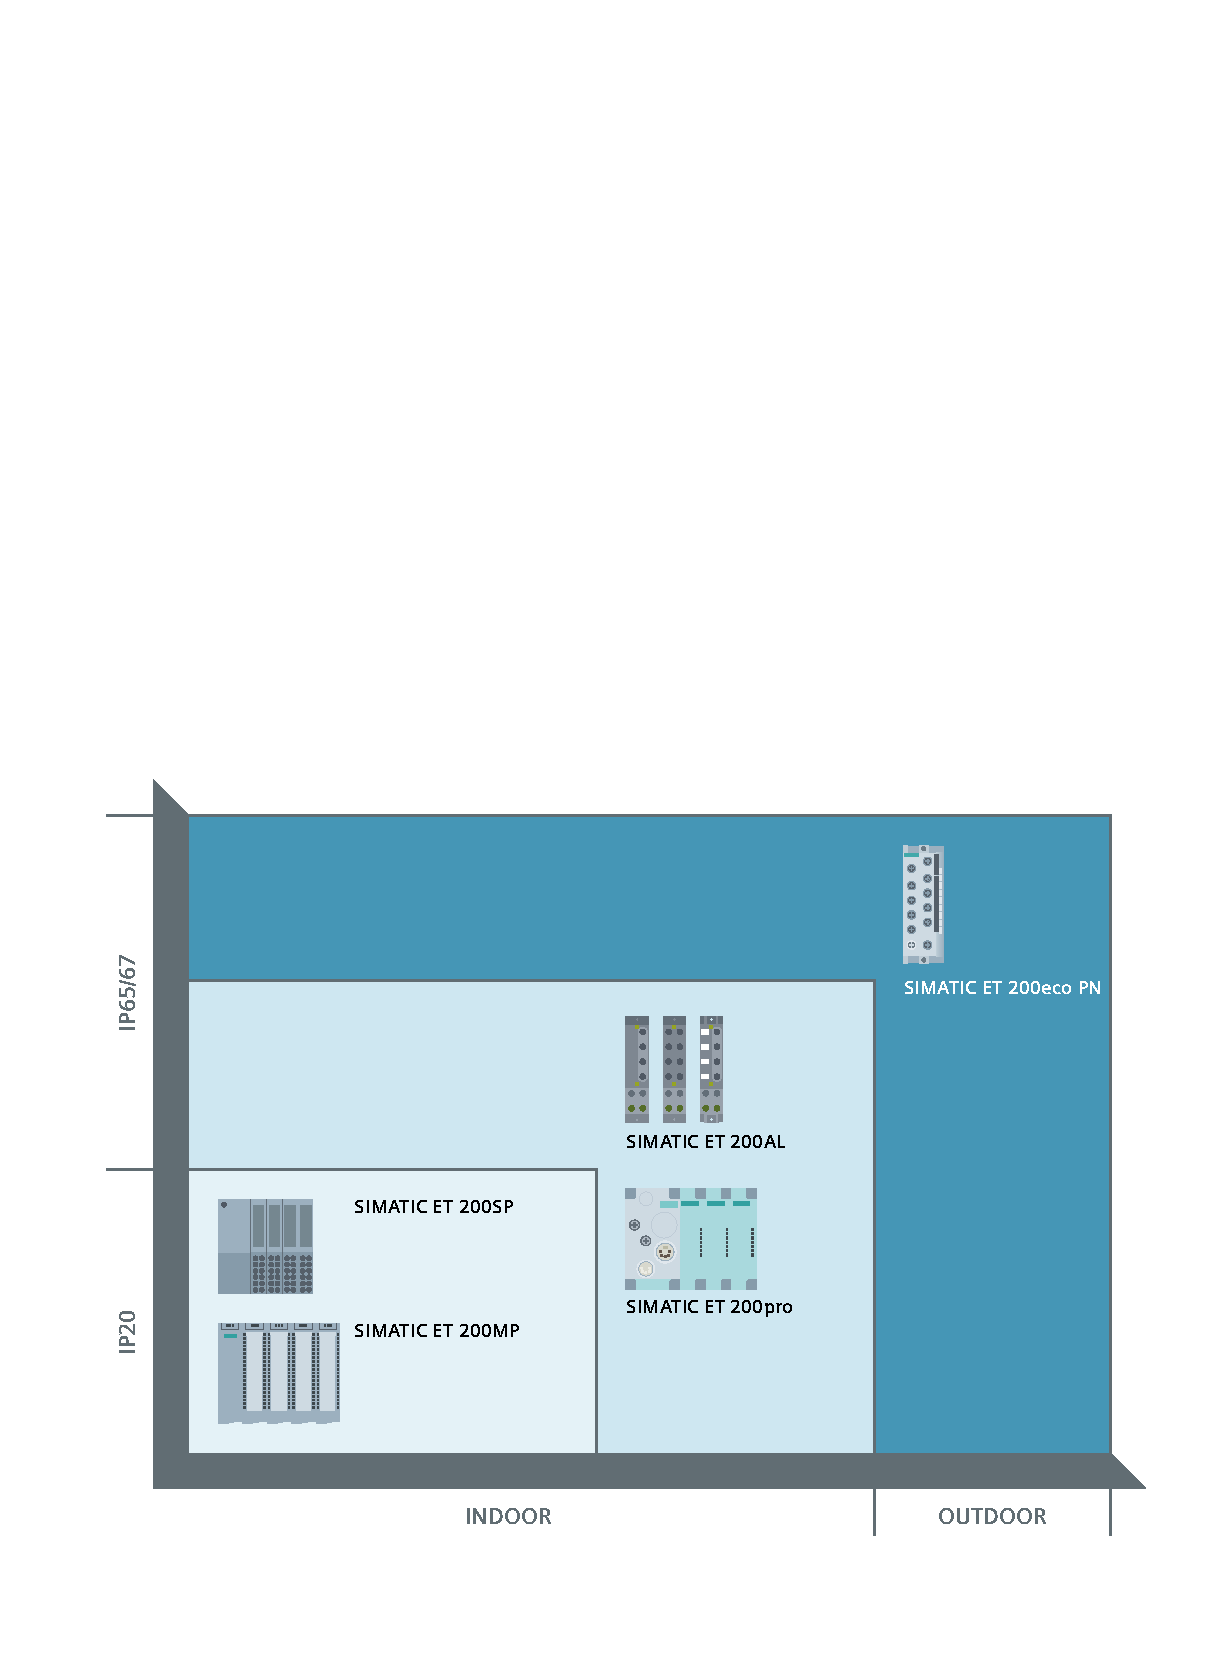
\includegraphics[width=0.87\textwidth]{assets/img/et200.pdf}
    \caption{Znázornění produktové řady SIMATIC ET 200}
    \source{Marketingové materiály firmy Siemens,~s.\,{}r.\,{}o. \cite{et200}}
    \label{fig:et200}
\end{figure}

Zařízení SIMATIC ET 200SP, které můžeme vidět na obrázku \ref{fig:et200sp}, je určeno k umístění do kompaktních řídících kabinetů. Díky modulárnosti systému se systém může vysoce přizpůsobit potřebám jednotlivých průmyslů. Mezi tyto moduly patří standardní I/O moduly, komunikační moduly, technologické moduly nebo moduly ke startování motorů. Zároveň je velikou výhodou celkový kompaktní design. Jednotlivé moduly zároveň mohou být vyměňovány za běhu. \cite{et200sp}

SIMATIC ET 200SP využívá tzv. Multifieldbus technologii. Tato technologie umožňuje zařízení komunikovat na základě několika průmyslových protokolů. V rámci této práce se zaměříme na protokoly ModbusTCP a EtherNet/IP, které již byli dříve popsané.

\begin{figure}[htbp]
    \centering 
    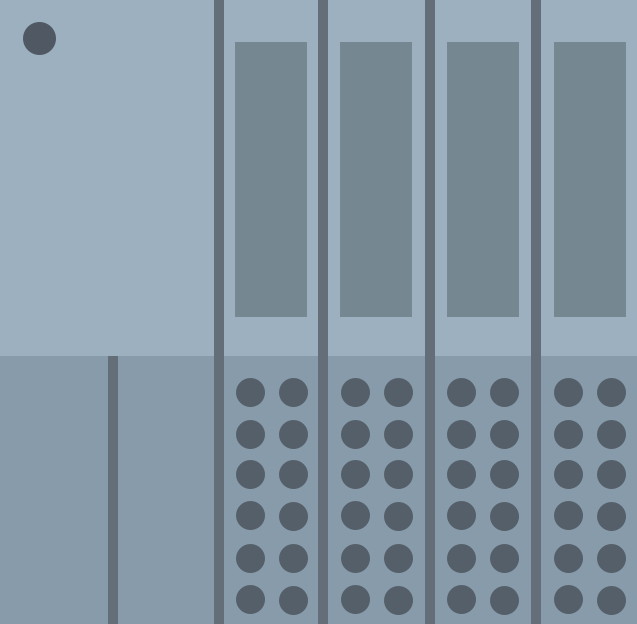
\includegraphics[width=\textwidth]{assets/img/et200sp.png}
    \caption{Zařízení SIMATIC ET 200SP}
    \source{Marketingové materiály firmy Siemens,~s.\,{}r.\,{}o. \cite{et200sp}}
    \label{fig:et200sp}
\end{figure}

\chapter{Návrh}

V této kapitole se budu věnovat návrhu knihovny na automatizaci a jejím funkčním požadavkům.

\section{Zařízení}
V rámci knihovny a testovacího běhu se bude vyskytovat několik účastníků. Tyto participanti budou:

\begin{description}
    \item[Testovací zařízení] Hlavní zařízení, ze kterého poběží testovací služba.
    \item[Fyzický participant] Fyzické zařízení, které běží mimo zařízení s testovací službou. 
    \item[Virtuální participant] Zařízení, které simuluje protistranu fyzickým participantům. Toto zařízení běží na stejném zařízení jako testovací služba.
\end{description}

Hlavním cílem je testovat vyvíjený produkt. V kontextu této knihovny ho budeme nazývat fyzický participant. Do této kategorie avšak také bude patřit jakékoliv zařízení, které běží mimo zařízení, které řídí testování. Tato zařízení budou k zařízení, které řídí testovaní, připojena za pomoci Ethernet připojení.

Knihovna zároveň bude obsahovat tzv. virtuálního participanta. Toto zařízení bude sloužit k simulaci protistrany u testování fyzického zařízení. Je to volitelný participant. Zároveň může být během testu připojeno více virtuálních participantů. Simulováním participanta snižujeme hardwarové nároky na testování, což vede ke snížení ekonomických nákladů na testování. Tito participanti se budou připojovat před započnutím určitého testu a po skončení tohoto jednoho testu zaniknou.

Testovací služba poběží na samostatném zařízení. Toto zařízení bude běžet na operačním systému Windows. Toto zařízení bude v rámci infrastruktury serveru Azure DevOps tzv. agent. Agent je výpočetní infrastruktura s nainstalovaným softwarem agenta, který pracuje na jedné určité úloze \cite{agent_docs}. Na agentovi bude server Azure DevOps spouštět testovací běh.

Testovací knihovna a virtuální participant budou vyvinuti v jazyce \inlinecode{C\#}. Jazyk byl vybrán kvůli dobrému rozsahu již implementovaných komponent a kvůli dobré interoperabilitě se serverem Azure DevOps, díky tomu že obě části jsou vyvíjeny společností Microsoft. Rozhraní pro vyvíjený produkt bude vytvořeno v jazyce \inlinecode{C++}, jelikož tento produkt je v tomto jazyce vyvíjen.


\section{Komunikace}
Komunikace mezi participanty bude fungovat na principu TCP/IP připojení. Zároveň zprávy, které budou mezi službou a participanty vyměňovány, budou mít stanovenou strukturu. Jedna zpráva bude obsahovat délku zprávy, typ zprávy a poté data zprávy. Data zprávy se budou odvíjet od typu zprávy. Existují i situace, kdy zpráva žádná data obsahovat nebude, k přenesení informace tedy bude stačit pouze typ zprávy. 

Složení zprávy lze vidět na obrázku \ref{fig:message}. Všechny hodnoty budou ukládány v kladné (anglicky tzv. unsigned) podobě. Z diagramu lze vidět, že jedna zpráva bude mít maximální délku rovna číslu, které se vejde do dvou bajtů, tedy maximální délka jedné zprávy je 65~535 bajtů. Tato délka je ale více než dostatečná pro navrhované použití.  

\begin{figure}[htbp]
    \centering 
    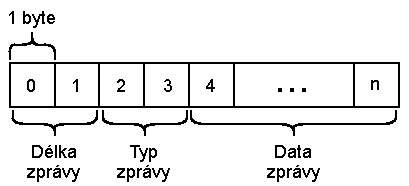
\includegraphics{assets/img/message.pdf}
    \caption{Diagram struktury jedné zprávy}
    \label{fig:message}
\end{figure}


\section{Testovací služba}
Ve vyvíjené knihovně bude jádrem k řízení testování služba, která se bude starat o běh testování. Služba v počáteční fázi vytvoří připojení se všemi fyzickými participanty testu. Po připojení určitého počtu očekávaných participantů započne samotné testování. Služba bude spouštět testy a během testu bude synchronizovat stádia testování mezi všemi participanty testu. Následně po běhu testu vyhodnotí úspěšnost testu na základě dat, které obdrží od participantů. 


\section{Rozhraní pro testování}
Součástí knihovny taktéž bude rozhraní, pro implementaci zařízení, které bude testováno. Toto rozhraní bude mít jasně definovanou  strukturu, ale zároveň bude co nejjednodušší pro co nejrychlejší implementaci na nově testovaném zařízení. Toto rozhraní bude potom využito pro řízení běhu testu na testovaném zařízení. 

Další součástí bude i rozhraní pro jednotlivé testy. To bude obsahovat jednotlivá stádia testování, která budou mezi všemi zařízeními synchronizovány. Tyto stádia budou, v tom pořadí:
\begin{enumerate}
    \item Příprava na testování
    \item Samotné testování
    \item Úklid po testu
\end{enumerate}

\section{Proces testování}

Ze předchozí definice testování vyplývá, že knihovna je mířena na automatizaci funkčního testování. Každý testovací běh se bude moc skládat z libovolného počtu registrovaných testů. Na obrázku \ref{fig:act_diag_device} můžeme vidět diagram aktivit testovaného zařízení. Samotné kontrolování správnosti testu bude prací jednotlivých testerů. Knihovna pouze dostane informaci o úspěchu nebo neúspěchu jednotlivých synchronizačních částí testovaní, definovaných rozhraním pro testování. Pokud ve fázi přípravy na testování nebo úklidu po testu zařízení vrátí neúspěch, bude toto zařízení považováno jako v chybném stavu. Další testy poté nebudou provedeny. 

\begin{figure}
    \centering 
    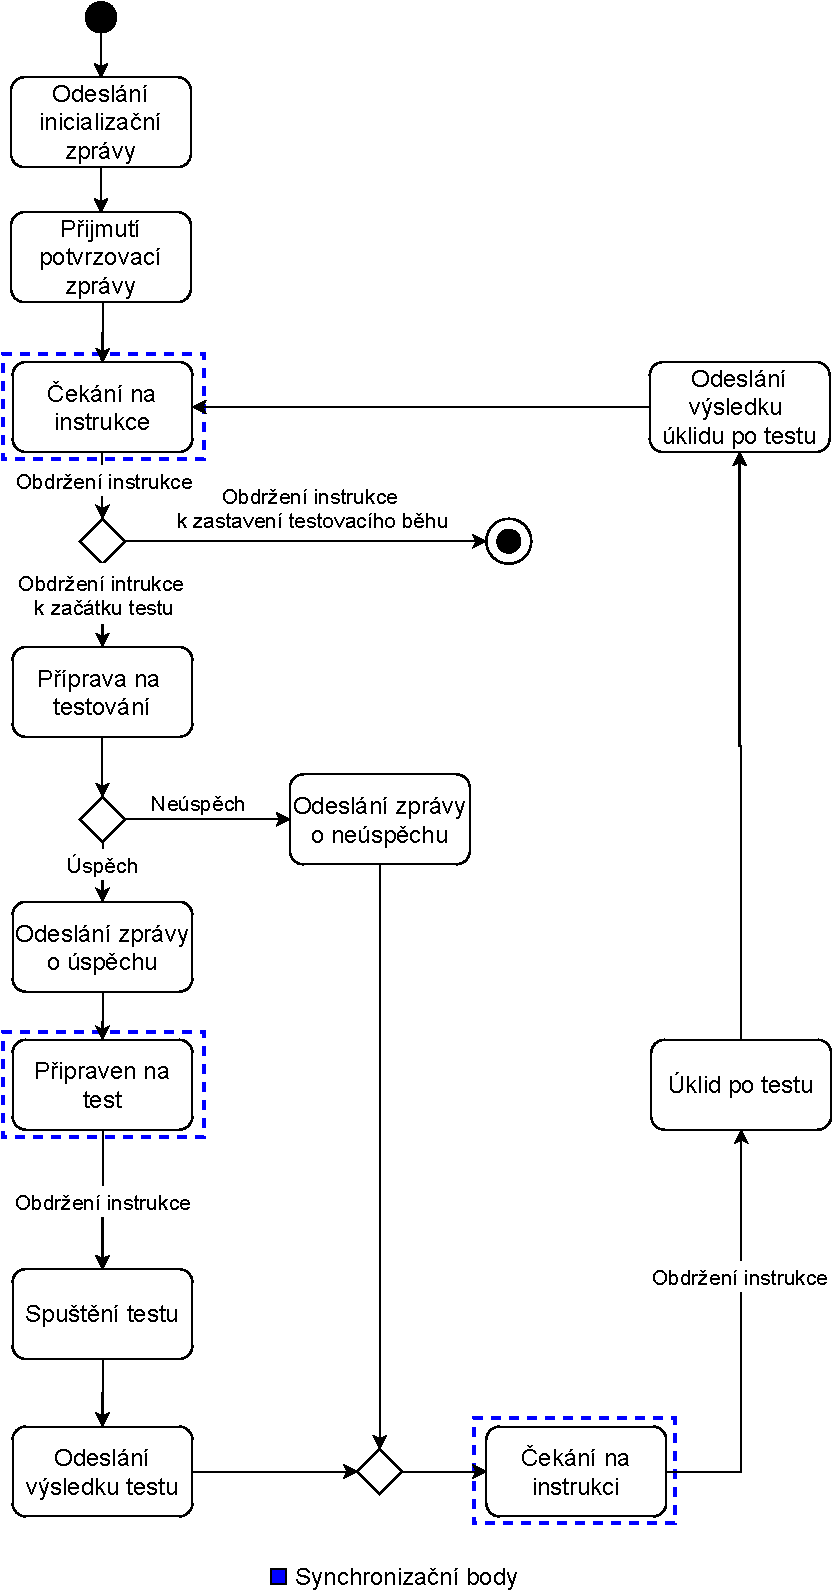
\includegraphics[width=\textwidth]{assets/img/activitydiagramdevice.pdf}
    \caption{Diagram aktivit testované zařízení}
    \label{fig:act_diag_device}
\end{figure}

\section{Propojení se serverem Azure DevOps}
Jedním z cílů této práce je vytvoření takového připojení, aby server Azure DevOps byl schopen spouštět jednotlivé testy. K tomuto propojení využijeme testovací framework MSTest. Vyvíjená testovací knihovna tedy poběží nad tímto testovacím frameworkem. Za pomoci frameworku MSTest bude server Azure DevOps schopen registrovat jednotlivé testy, a spouštět je jednotlivě.



\chapter{Implementace}

Tato kapitola se věnuje implementační části všech navrhnutých komponent, které umožnují automatizaci testování.

\section{Komunikace}
Testovací knihovna má jasně definovanou komunikaci. Strukturu jedné zprávy zajišťuje třída \inlinecode{Message}. Dle návrhu má jedna odeslaná zpráva definované tři atributy -- délku zprávy, typ zpráva a data zprávy. Třída \inlinecode{Message} si drží dva z těchto atributů, třetí -- délka zprávy -- je na základě ostatních dvou vypočítána. Typ zprávy je určen enumerátorem \inlinecode{MessageType}. Tento enumerátor obsahuje výčty:

\begin{itemize} 
    \item \inlinecode{MSG\_FAIL} -- zpráva o neúspěchu
    \item \inlinecode{MSG\_OK} -- zpráva o úspěchu nebo potvrzení
    \item \inlinecode{MSG\_RUNTEST} -- pokyn k započnutí testu
    \item \inlinecode{MSG\_STOP} -- pokyn k ukončení testování
    \item \inlinecode{MSG\_EXCEPTION} -- chybná zpráva, slouží pro rozpoznání neplatné zprávy
\end{itemize}

Data zprávy jsou uložena v dynamickém poli. 

\todo{Doplnit}


\section{Testovací služba}
Jak již bylo zmíněno, jádrem k ovládání testování je testovací služba. V implementaci je tento celek rozdělen na dvě hlavní třídy. Třída \inlinecode{TestService} obstarává jednotlivé úkony služby, následně třída \inlinecode{ServiceRunner} propojuje třídu \inlinecode{TestService} s ostatními komponentami, které jsou potřebné pro testování.

\subsection{Nastavení služby}

Konfigurace služby je uložena v souboru \inlinecode{config.xml}. Tento soubor obsahuje tři hodnoty pro nastavení:

\begin{itemize}
    \item \inlinecode{ip} -- Adresa, na které bude služba poslouchat příchozí připojení. Všechna zařízení se budou připojovat na tuto adresu.
    \item \inlinecode{port} -- Síťový port, skrz který služba provádí komunikaci
    \item \inlinecode{participants} -- Počet fyzických participantů, které se připojí ke službě.   
\end{itemize}

Ukázku tohoto souboru můžeme vidět na výpisu \ref{listing:configxml}. V knihovně se o konfiguraci stará třída \inlinecode{Configuration}. Tato třída existuje v jmenném prostoru \inlinecode{GlobalVar}. Tento jmenný prostor simuluje globální proměnnou. Kvůli tomu jsou ale všechny třídy, které jsou odsud používány, konstruovány tak, aby primárně fungovaly jen ke čtení. Při vytvoření instance třída získá konfiguraci z konfiguračního souboru a uloží je do vnitřních proměnných třídy. Tyto proměnné jsou určeny pouze ke čtení, nelze je upravovat. Stav konfigurace určuje proměnná \inlinecode{bool IsValid}. V případě chyby je tato proměnná nastavená na hodnotu \inlinecode{false} a v proměnné \inlinecode{Exception} je uložen důvod neúspěchu. V opačném případě je tato proměnná nastavena na hodnotu \inlinecode{true}.

\begin{listing}[htbp]
    \centering
    \begin{minted}{xml}
        <?xml version="1.0" encoding="UTF-8" ?>
        <configuration>
          <!-- IP of the service-->
          <ip>192.168.4.100</ip>
          <!-- Port of the service -->
          <port>1337</port>
          <!-- Number of non-virtualized participants-->
          <participants>1</participants>
        </configuration>
    \end{minted}
    \caption{Ukázka konfiguračního souboru}
    \label{listing:configxml}
\end{listing}


\subsection{Operace služby}

Jak jsem již zmínil, jednotlivé úkony služby jsou implementovány v třídě \inlinecode{TestService}. Třída po své konstrukci inicializuje vnitřní proměnné, ale neprovádí žádné úkony. 

\subsubsection{Odesílání a přijímání zpráv}
Struktura jedné zprávy je již známým faktem. O jednotlivá připojení se avšak stará třída \inlinecode{TestService}. Třída má dvě hlavní statické metody pro odesílání a přijímání jednotlivých zpráv. Tyto metody jsou:

\begin{itemize}
    \item \inlinecode{static void SendMessage(TcpClient client, Message msg)} \\
    Metoda pro odeslání zprávy jednomu klientovi
    \item \inlinecode{static bool RcvMessage(TcpClient client, out Message msg)} \\
    Metoda pro přijmutí zprávy od jednoho klienta
\end{itemize}

Všechny zprávy jsou následně odesílány a přijímány za pomoci těchto dvou metod. Rozšířením těchto metod jsou metody \inlinecode{SendParticipantsMessage} a \inlinecode{CheckParticipantsResponse}. Obě metody pracují se všemi participanty připojenými ke službě. Metoda \inlinecode{SendParticipantsMessage} odešle všem participantům jednu zprávu, naopak metoda \inlinecode{CheckParticipantsResponse} zprávu od všech participantů přijme a zkontroluje, zda se všechny typy zprávy shodují s očekávaným typem zprávy. Očekávaný typ zprávy je předán v argumentu metody. \todo{CheckParticipantsResponse co vrací}

\subsubsection{Inicializace}

Metodou \inlinecode{bool Init(int InitTimeout)} třída \inlinecode{TestService} inicializuje běh služby. Proměnná \inlinecode{InitTimeout} určuje dobu, kdy služba čeká na příchozí komunikaci. Doba je metodě předávána, stejně jako všem ostatním metodám, které mají definovaný časový limit, v milisekundách. 

Metoda z konfigurace zjistí IP adresu a port, na kterém má služba běžet. Následně začne na této IP adrese a portu poslouchat příchozí komunikaci. V této fázi se připojují pouze fyzická zařízení. Z nastavení služba ví, kolik participantů má očekávat. 

V případě příchozí komunikace je poté zavolána metoda \inlinecode{AddClient}. Tato metoda vytvoří klienta a přijme identifikační zprávu od participanta. Tato zpráva má typ zprávy \inlinecode{MSG\_OK} a v datech zprávy obsahuje MAC adresu participanta. Metoda odešle participantovi potvrzovací zprávu s typem zprávy \inlinecode{MSG\_OK}, bez dat. 

Po úspěšném ověření připojení metoda uloží vytvořeného klienta a jeho MAC adresu do seznamu připojených participantů. Metoda zároveň rozezná připojení virtuálního participanta. Tento participant má MAC adresu \inlinecode{DE:AD:BE:EF:00:00}. Nakonec metoda vrací tři hodnoty typu integer:
\begin{itemize}
    \item \inlinecode{0} -- pokud připojování participanta vyústilo v neúspěch, ať už kvůli překročení časového limitu, nebo kvůli nedodržení stanovené komunikace.
    \item \inlinecode{1} -- pokud služba úspěšně přijme fyzického participanta
    \item \inlinecode{2} -- pokud služba úspěšně přijme virtuálního participanta
\end{itemize}

Služba úspěšně ukončuje inicializační fázi poté co se úspěšně připojí stejný počet participantů, jako bylo určeno v konfiguraci. V případě nepřipojení se očekávaného počtu zařízení v definovaném čase, obdržení špatné nebo žádné zprávy služba vyhodnocuje inicializační fázi jako neúspěšnou. Připojení virtualizovaného participanta v této fázi vyústí též v neúspěch inicializace.

\subsubsection{Spuštění testu}

Nejpodstatnější operací je spuštění jednotlivých testů. O toto se stará metoda \inlinecode{TestResult RunTest<T>(T testEnum, int timeout)}. Metoda očekává dva parametry:

\begin{itemize}
    \item \inlinecode{T testEnum} -- Identifikátor testu s generickým identifikátorem T, který typem musí být enumerátor.
    \item \inlinecode{int timeout} -- Maximální délka, po kterou služba očekává odpověď od participantů testu. 
\end{itemize}

Pro započnutí testu na testovaném zařízení služba odešle zprávu, s typem zprávy \inlinecode{MSG\_RUNTEST}. Data této zprávy obsahují:

\begin{enumerate}
    \item Číselnou reprezentaci enumerátoru \inlinecode{testEnum}. Ten je uložen v prvních 4 bytech dat zprávy.
    \item Číselnou reprezentaci enumerátoru \inlinecode{TestStateE}, určující stádium testování. Uložen je ve dvou bajtech dat zprávy hned za identifikátorem testu.
\end{enumerate}

Tato metoda postupně spouští všechny stádia testování. Tyto stádia jsou rozlišovány za pomocí emulátoru \inlinecode{TestStateE}. Jednotlivě:

\begin{itemize}
    \item \inlinecode{TEST\_STARTUP} -- příprava na testování
    \item \inlinecode{TEST\_RUN} -- spuštění testu
    \item \inlinecode{TEST\_TEARDOW} -- úklid po testu
\end{itemize}

Po spuštění jednotlivých stádií testování metoda čeká na odpověď od všech participantů. Participant odesílá službě zprávu s typem \inlinecode{MSG\_OK} pro úspěch, a nebo s typem \inlinecode{MSG\_FAIL} pro neúspěch. Obě zprávy neobsahují žádné data.

Doba čekání je určena argumentem \inlinecode{timeout}. Tento čas je vázaný na jednotlivá stádia testování. Tedy pokud metoda má časový limit 30 sekund, tak poté bude po každém stádiu testování čekat 30 sekund na odpověď od participanta. V případě že vyprší časový limit, tak je participant považován jako v chybném stavu. Taktéž je participant považován jako v chybném stavu, pokud vrátí neúspěch u přípravy na testování nebo u úklidu po testu.

Metoda následně vrací jednotu z hodnot enumerátoru \inlinecode{TestResult}. Tyto hodnoty jsou:

\begin{itemize}
    \item \inlinecode{TEST\_SUCCESS} -- test proběhl úspěšně
    \item \inlinecode{TEST\_FAIL} -- test proběhl neúspěšně
    \item \inlinecode{TEST\_ERROR} -- v průběhu testování se vyskytla chyba a další testování není možné   
\end{itemize}


\subsubsection{Ukončení testování}

Po dokončení celého testovacího běhu je zavolána metoda \inlinecode{Stop()}. Tato metoda odešle všem participantům stále připojeným ke službě zprávu s typem \inlinecode{MSG\_STOP} a ukončí spojení. Testování avšak může být ukončeno i v případě vzniklé chyby. Služba se snaží v případě chyby ukončit co nejvíce zařízení skrz stanovený protokol.

\subsubsection{Virtuální participanti}

Jelikož každý test může obsahovat různý počet virtuálních participantů, je podstatné, aby služba mohla při testovacím běhu tyto participanty přidávat a odebírat. K tomuto slouží dvě metody. Metoda \inlinecode{AddVirtualParticipant} řekne službě, že má očekávat připojení virtuálního participanta. V případě úspěšného připojení virtuálního participanta služba vrací úspěch. Naopak případě chyby, nebo připojení fyzického participanta, metoda vrací neúspěch. O opačnou operaci se stará metoda \inlinecode{StopVirtualDevices}. Metoda po svém zavolání odešle všem virtuálním participantům zprávu o ukončení testování a tato zařízení jsou odpojena a ukončena.

\subsection{Propojení s ostatními komponentami}

O propojení třídy \inlinecode{TestService} s ostatními komponentami knihovny se stará třída \inlinecode{ServiceRunner}.
Tato třída ve svém konstruktoru inicializuje konfiguraci služby a zjistí, zda je validní. Tento konstruktor přijímá jeden argument -- časový limit na inicializaci. V případě nezadání tohoto parametru třída využije defaultní časový limit definovaný ve třídě na 60 sekund. Následně konstruktor vytvoří instanci třídy \inlinecode{TestService} a zavolá metodu \inlinecode{Init}. V případě jakékoliv chyby je služba vyhodnocena jako v chybovém stavu. Toto určuje enumerátor \inlinecode{RunnerState}, který má dvě možné hodnoty: 

\begin{itemize}
    \item \inlinecode{ERROR} -- služba je v chybovém stavu
    \item \inlinecode{OK}  -- služba je v pořádku  
\end{itemize}

Tato informace je uložena ve vlastní proměnné \inlinecode{State}. Následný důvod vyhodnocení chyby je uloženo v proměnné \inlinecode{Exception}. Třída následně má další metody, skrz které umožňuje ovládání instance třídy \inlinecode{TestService}. Tyto metody jsou:

\begin{itemize}
    \item \inlinecode{bool RunTest<T>(T test, int timeout = DefaultTimeout)} \\ Metoda předá instrukci pro spuštění testu. Očekává stejné parametry jako metoda \inlinecode{RunTest} třídy \inlinecode{TestService}. Jedinou změnou je, že pokud časový limit nebude zadán, tak bude použit defaultní časový limit.
    \item \inlinecode{bool AddVirtualParticipant()} \\ Metoda předá informaci o očekávání připojení virtuálního participanta.
    \item \inlinecode{void TestCleanup()} \\ Metoda je volána po dokončení jednotlivého testu. V aktuální implementaci třída předá informaci o požadavku na odpojení virtuálních participantů.
    \item \inlinecode{void Stop()} \\ Metoda předá informaci o ukončení testovacího běhu.
\end{itemize}


\section{Rozhraní pro testovaná zařízení}

Rozhraní pro testovaná zařízení umožňuje propojení s testovací službou. Jeho cílem je být co nejjednodušší pro co nejrychlejší implementaci. Definici rozhraní pro jazyk \inlinecode{C++} můžeme vidět na výpisu \ref{listing:dev_if}.

\begin{listing}[htbp]
    \begin{minted}[breaklines]{cpp}
    class DeviceIf
    {
    public:

        virtual ~DeviceIf() {}

        virtual bool createConnection(const char * ipAddress, uint16_t port) = 0;

        virtual bool sendMessage(const Message& msg) = 0;

        virtual bool rcvMessage(Message& msg) = 0;

        virtual TestCaseIf * getTest(uint32_t test) = 0;

        virtual bool getMacAddress(uint8_t** macAddr, uint32_t* size) = 0;
    };
    \end{minted}
\caption{Ukázka definice rozhraní}
\label{listing:dev_if}
\end{listing}

\todo{Dopsat}


\section{Virtuální participant}
Implementace virtuálního participanta přímo kopíruje navrhnuté rozhraní pro testované zařízení. Logika virtuálního participanta je obsažena ve třídě \inlinecode{VirtualClient}. Tato třída tři možné konstruktory:

\begin{itemize} 
    \item \inlinecode{VirtualClient(ITestClient device)} \\
    Konstruktor dostane v argumentu odkaz na implementaci rozhraní zařízení
    \item \inlinecode{VirtualClient (ITestCase testCase)} \\
    Konstruktor dostane v argumentu odkaz na implementaci jednoho testu, který je odvozený z rozhraní pro test.
    \item \inlinecode{VirtualClient (Func<UInt32, ITestCase> getTest)} \\
    Argumentem konstruktoru je funkce, která obsahuje seznam testů. Funkce v argumentu dostane číselnou reprezentaci testu a vrací instanci testu, který je odvozený z rozhraní testu.
\end{itemize}

Třída následně vytvoří instanci implementace rozhraní klienta. Tato implementace je obsažena ve třídě \inlinecode{TestClientDefault}. Testovací běh virtuálního participanta funguje na stejném principu jako běh ostatních testovaných zařízení. Rozdílem je, že třída \inlinecode{VirtualClient} vytvoří nové vlákno, na kterém běží tento virtuální participant. Vytvořené vlákno (a s ním i virtuální participant) je poté spuštěno metodou \inlinecode{Start}. Následně metoda \inlinecode{Stop} ukončuje běh virtuálního participanta. Metoda nejdříve čeká, zda se participant a vlákno ukončí standardním způsobem. Pokud se virtuální participant neukončí ve stanoveném časovém limitu, tak ho metoda ukončí ukončením běžícího vlákna.
\todo{Doplnit}


\section{Propojení s frameworkem MSTest}

Podstatnou součástí implementace je propojení služby s testovacím frameworkem MSTest. O toto se stará třída \inlinecode{API}. Jako jediná třída využívá nástroje tohoto frameworku. Třída je koncipovaná jako statická třída, i když je závislá na jím vytvořené instanci třídy \inlinecode{ServiceRunner}. Toto je uděláno z důvodu designového omezení frameworku MSTest. 

Při spuštění jednotlivých testů je nutné brát v potaz, že testovací služba neví jaké testy budou kdy spuštěny. Testovací služba se tedy musí používat nezávisle na těchto testech. K tomuto využijeme dvě funkce frameworku MSTest -- \inlinecode{AssemblyInitialize} a \inlinecode{AssemblyCleanup}. Tyto dvě funkce jsou spuštěny ještě před započnutím a po skončení testovaní. V třídě \inlinecode{API} jejím implementacím odpovídají metody \inlinecode{AssemblyInit} a \inlinecode{AssemblyCleanup}. Metoda \inlinecode{AssemblyInit} přijímá dva argumenty:

\begin{itemize}
    \item \inlinecode{Assembly assembly} -- odkaz na runtime blok, který reprezentuje spuštěný blok programu mimo knihovnu
    \item \inlinecode{int InitTimeout} -- časový limit na inicializační fázi služby (tedy časový limit, který je využíván v metodě \inlinecode{TestService.Init}), pokud je ponechán prázdný, je použit defaultní časový limit z třídy \inlinecode{ServiceRunner}.
\end{itemize}

Předání runtime bloku -- neboli assembly -- je sice dobrovolným krokem, ale podstatným. Při odesílání testů služba odesílá pouze číselnou reprezentaci enumerátoru, který test identifikuje. Tento enumerátor ale nemusí být stejného typu. Proto zde může vzniknout kolize.

Framework MSTest využívá pro rozlišení testovacích součástí tzv. atributy. Atributy přidávají metadata k třídám, typům, metodám atd. \cite{attribute_docs}. Framework MSTest využívá například tyto atributy:

\begin{itemize}
    \item \inlinecode{AssemblyInitialize} -- identifikuje inicializační funkci
    \item \inlinecode{AssemblyCleanup} -- identifikuje funkci která bude spuštěna po skončení všech testů
    \item \inlinecode{TestClass} -- identifikuje třídu, která obsahuje testy
    \item \inlinecode{TestMethod} -- identifikuje metody, které reprezentují jednotlivé testy
\end{itemize}

Testovací knihovna tuto sadu atributů rozšiřuje o atribut \inlinecode{TestEnum}. Tento atribut říká, že enumerátor s atributem \inlinecode{TestEnum} reprezentuje nějaké testy. Proto metoda \inlinecode{AssemblyInit} prostřednictvím argumentu \inlinecode{assembly} zjistí, které enumerátory mají tento atribut. Následně zkontroluje, zdali tyto enumerátory nemají mezi sebou kolize. V případě nalezení kolize je vyhozena výjimka. Tato kontrola se dá přeskočit předáním hodnoty \inlinecode{null} v argumentu \inlinecode{assembly}.

Metoda \inlinecode{AssemblyCleanup} symetricky ukončuje běh testovací služby. V určitých případech tato funkce nemusí být zavolána \question{Je zde potřeba citace}. Při zjištění chyby v běhu, která vyústí v ukončení testovacího běhu, je tato funkce volána manuálně.

Pro spuštění testování je použita metoda \inlinecode{Run}. Tato metoda přijímá stejné argumenty jako metoda \inlinecode{RunTest} třídy \inlinecode{ServiceRunner}. Metoda zkontroluje, že argument identifikující test je typem enumerátor a obsahuje atribut \inlinecode{TestEnum}. V případě že se testovací služba nenachází v chybném stavu, tak metoda předá testovací službě direktivu k započnutí testu. Následně vyhodnotí úspěšnost testu. V případě, že služba je v chybném stavu, metoda vyhodnotí test jako bezvýsledný. 
 

\chapter{Průzkum open-source knihoven pro průmyslové protokoly}

\dummytext{1-10}

\chapter{Vyhodnocení vytvořeného řešení}\label{chap:evaluation}

\note{Tato kapitola je stále ve vývoji}

\begin{conclusion}
Cílem této práce bylo vytvořit testovací knihovnu, která umožní automatizovat testy verifikace průmyslové komunikace. Tato knihovna následně měla být propojena s Azure DevOps serverem tak, aby Azure DevOps server mohl automaticky testy spouštět, vyhodnocovat a poskytovat uživateli informace o průběhu jednotlivých testů. Dalším cílem práce bylo prozkoumat dostupné open-source knihovny pro průmyslové protokoly ModbusTCP a EtherNet/IP a za pomoci jedné z knihoven demonstrovat funkcionalitu vytvořeného řešení. V neposlední řadě bylo cílem zhodnotit vytvořené řešení a jeho přínosy.

Cíle této práce byly splněny. Práce v kapitole \ref{chap:teorie} definuje jednotlivé pojmy a přibližuje kontext této práce. Testovací knihovna a všechny její části byly následně v kapitole \ref{chap:design} navrhnuty. Testovací služba, která řídí testovací běh, byla navrhnuta jako doplněk do testovacího frameworku MSTest. Následně za pomoci tohoto frameworku bylo řešení propojeno s Azure DevOps, který mohl jednotlivé testy registrovat, automaticky spouštět a zobrazovat jejich výsledky. Implementace všech částí testovací knihovny byla následně popsána v kapitole \ref{chap:implementation} a funkčnost vytvořeného řešení demonstrována v kapitole \ref{chap:demonstration}. Kapitola \ref{chap:evaluation} následně zhodnotila vytvořené řešení, jeho přínosy a úskalí. 

Vytvořené řešení splňuje požadavky, které na něj byly kladeny, avšak je zde stále prostor pro zlepšení. Zřejmým rozšířením knihovny je implementace jednotlivých testovacích partnerů, kteří budou simulovat chování jednotlivých zařízení. Zároveň je možné zlepšit registraci testů, respektive automatizovat tuto registraci, na testovaném zařízení. 
\end{conclusion}


{
    \setlength{\emergencystretch}{3em} 
    \printbibliography
}

\appendix

\chapter{Seznam použitých zkratek}
\begin{description}
	\item[Ethernet/IP] Ethernet Industrial Protocol
	\item[I/O] Input/Output
	\item[IDE] Integrated Development Environment 
	\item[IP] Internet Protocol 
	\item[PDU] Protocol Data Unit 
	\item[PLC] Programmable Logic Controller
	\item[TCP/IP] Transmission Control Protocol/Internet Protocol 
	\item[XML] Extensible markup language
\end{description}

\chapter{Seznam zdrojů cen zařízení a licencí}\label{chap:price_list}

V tabulce \ref{tab:device_prices} lze vidět seznam zařízení, jejich cenu a zdroj ceny. Ceny byli získány 16.04.2021 a případně převedeny do českých korun dle kurzu k tomuto dni.

\begin{table}[H]
    \centering
    \resizebox{\textwidth}{!}{
    \begin{tabular}{|C{4cm}|C{2.5cm}|C{10.5cm}|}\hline
        \textbf{Produkt} & \textbf{Cena za kus bez DPH} & \textbf{Zdroj} \\\hline
        Beckhoff CX2030-0125 &  \koruna{66650.44} &  \url{https://www.radwell.co.uk/Buy/BECKHOFF/BECKHOFF/CX2030-0125}\\\hline
        Beckhoff CX2100-0004 &  \koruna{8663.21} &  \url{https://www.radwell.co.uk/en-GB/Buy/BECKHOFF/BECKHOFF/CX2100-0004/} \\\hline
        Schneider Electric BMXP342020 340-20  & \koruna{30536.8} & \url{https://cz.farnell.com/schneider-electric/bmxp342020/processor-module-0-095a-24vdc/dp/2835381} \\\hline
        Schneider Electric BMXCPS2000 &  \koruna{5220.27} &  \url{https://cz.rs-online.com/web/p/prislusenstvi-pro-plc/0148026/} \\\hline
        Schneider Electric BMXXBP0400 &  \koruna{3493.03} &  \url{https://uk.rs-online.com/web/p/plc-accessories/0147922/}  \\\hline
        Schneider Electric M251MESC &  \koruna{8192.46} &   \url{https://cz.rs-online.com/web/p/plc-programovatelne-logicke-kontrolery/8066755/} \\\hline
        Schneider Electric TM262L20MESE8T &  \koruna{36636.86}  &  \url{https://at.rs-online.com/web/p/sps-zentralbaugruppen/2011448/} \\\hline
        Rockwell Automation 1769-L24ER-QB1B &  \koruna{38526.54} & \url{https://www.routeco.com/en-gb/shop/programmable-controllers/compactlogix/1769-l24er-qb1b} \\\hline
        Rockwell Automation 1783-BMS20CGN & \koruna{64480.27} &  \url{https://cz.wiautomation.com/allen-bradley/industrial-communication/stratix/1783BMS20CGN} \\ \hline
        Schneider Electric Machine Expert & \koruna{23987.18} & \url{https://cz.wiautomation.com/schneider-electric/software/ESECAPCZZSPMZZ} \\\hline
        Schneider Electric SO Machine & \koruna{26907.28} & \url{https://www.alliedelec.com/product/schneider-electric/somnacczxspazz/70596759} \\\hline
        Rockwell Automation Studio 5000 & \koruna{79140.18} &  \url{https://twcontrols.com/lessons/where-can-i-download-studio-5000-logix-designer-rslogix-5000-and-what-is-the-pricedifference-of-each-version}\\\hline
        Schneider Electric Unity Pro & \koruna{102299.92} &  \url{https://cz.wiautomation.com/schneider-electric/software/UNYUPDSPUXUG} \\\hline
    \end{tabular}
    }
    \caption{Seznam zdrojů cen zařízení a softwarových licencí}
    \label{tab:device_prices}
\end{table}

\chapter{Obsah přiložené SD karty}

\begin{figure}
	\dirtree{%
		.1 readme.txt\DTcomment{stručný popis obsahu SD karty}.
		.1 package\DTcomment{adresář se zkompilovaným balíčkem testovací knihovny}.
		.1 impl\DTcomment{zdrojové kódy implementace}.
		.2 cpp\DTcomment{implementace pro testované zařízení v jazyku \cpp{}}.
		.2 core\DTcomment{implementace jádra testovací knihovny v jazyku \csharp{}}.
		.2 test\_project\DTcomment{testovací projekt vytvořený k demonstraci funkčnosti}.
		.1 text\DTcomment{text práce}.
		.2 src\DTcomment{zdrojová forma práce ve formátu \LaTeX{}}.
		.2 thesis.pdf\DTcomment{text práce ve formátu PDF}.
	}
\end{figure}

\end{document}
